% Racing the Scanner: final report (#60).
% Every number below is derived from this repository: the regenerated figures
% (scripts/run_demo.sh), captured/*.csv, results/*.csv, and docs/. See README.md.
\documentclass[conference]{IEEEtran}
\usepackage[T1]{fontenc}  % for the ogonek in M\k{a}dry
\usepackage{graphicx}
\usepackage{booktabs}
\usepackage{amsmath}
\usepackage{url}
\usepackage{cite}
\graphicspath{{figures/}}

\begin{document}

\title{Racing the Scanner: Detection Loses to Mimicry,\\a CPU Reservation Sidesteps It}

\author{\IEEEauthorblockN{Muhammad Abdullah Hasnain, Muhammad Abdullah Khan, Syed Ibad Asim}
\IEEEauthorblockA{Dhanani School of Science and Engineering, Habib University, Karachi}}

\maketitle

\begin{abstract}
A live RAM scanner catches a process that hides its memory only during the few
milliseconds the process exposes a page, so whether it catches the process at
all depends on whether the scheduler lets it run in time. We study an attacker
that hides its memory, starves the scanner of CPU, and shapes its own timing to
look like a benign application (mimicry). We simulate 20 scheduling policies:
stock EEVDF, 14 machine-learning policies that detect and demote the hog (a
fifteenth, an autoencoder, needs PyTorch and is excluded), four standard Linux
reservations, and a reservation floor we call the invariant. Every evaluated ML
policy is evaded: the scanner misses 100\% of its exposure windows (median of
20 runs; single runs of three policies dip to 0.78--0.98). The detectors barely
see the disguised hog: 11 of the 14, and the family median ROC-AUC against
benign apps (0.285), sit at or below chance, and the three that rank it slightly
above chance (0.55--0.61) never demote it. Every CPU reservation keeps the
scanner on time (0\% miss) without classifying any process, at 5.8$\times$ to
826$\times$ less policy compute than the ML policies. Cgroup \texttt{cpu.weight}
and \texttt{SCHED\_DEADLINE} are numerically identical to our invariant, which
is therefore one instance of a standard primitive, not a new one. On a real
Linux~7.0 kernel, a nice~$-20$ CPU hog slows the scanner 9.1$\times$ under stock
EEVDF, while \texttt{cpu.weight} and \texttt{SCHED\_FIFO} hold it at the
no-attack rate. A custom Tracee rule catches 15 of 15 hiding processes with 0 of
30 false alarms, where Tracee's default signatures catch none. The contribution
is a validated reframing: do not try to win the detection arms race; sidestep it.
\end{abstract}

\begin{IEEEkeywords}
CPU scheduling, CPU reservation, cgroups, sched\_ext, EEVDF, memory scanning,
mimicry attacks, eBPF, Tracee.
\end{IEEEkeywords}

\section{Introduction}
Memory scanners find malware by matching byte patterns in a process's memory.
An attacker can defeat a scanner by keeping its payload encoded or unmapped and
exposing one page at a time, for a few milliseconds, only when it needs it. A
live scanner then catches the payload only if a scan lands inside an exposure
window. That makes detection a race for CPU: if the attacker can also delay the
scanner, by claiming a high priority and hogging the core the scanner runs on,
the scans arrive too late to see anything.

A scheduler can defend the scanner in two ways. It can \emph{detect} the
attacker and demote it, which is what an ML-augmented scheduler does; or it can
\emph{reserve} CPU for the scanner without judging anyone. We compare three
families: the stock Linux scheduler (EEVDF~\cite{eevdf,lwn-eevdf}), 14
machine-learning policies that score every process and demote a suspected hog,
and five reservations (\texttt{SCHED\_FIFO}, cgroup \texttt{cpu.max} and
\texttt{cpu.weight}~\cite{cgroupv2}, \texttt{SCHED\_DEADLINE}~\cite{lelli-deadline},
and an invariant floor of our own).

\textbf{Thesis.} Against an attacker that disguises its timing, scheduling that
works by detecting the attacker fails: the disguised hog looks at least as
benign as the benign apps (11 of 14 detectors, and their median, score it at or
below chance), so every one of the 14 evaluated ML policies leaves the scanner
starved (100\% median miss). What keeps the scanner running is a structural
reservation that classifies no one, at 5.8$\times$ to 826$\times$ less policy
compute, and that reservation is a standard primitive. The idea is not new: adaptive
adversaries defeat detectors built for a fixed attacker~\cite{wagner-mimicry,
biggio-wild,tramer-adaptive}, and reservations are the classic answer to
resource contention~\cite{rajkumar-resource-kernels}. Our contribution is the
reframing and its validation for this attack: a reproducible simulation across
20 policies, real-kernel runs that confirm the reservation half on hardware, a
detection study with Tracee~\cite{tracee}, and an honest account of what each
piece does and does not show.

This framing is itself a correction: an earlier version presented our invariant
as a unique mechanism, until the standard Linux reservations, added as
baselines, matched it exactly (issues \#28/\#29).

\section{Methods}

\subsection{Threat model}
The defender is a live RAM scanner that reads a target's memory through
\texttt{/proc/<pid>/mem} and looks for a known marker. The attacker holds a
1~MB buffer of that marker and hides it with one of four payloads. To delay the
scanner it also runs CPU-bound work on the scanner's core at a claimed high
priority. Four conditions separate the two halves of the attack: \emph{none},
\emph{hiding} (hides, does not hog), \emph{starvation} (hogs, does not hide),
and \emph{coupled} (both). In the simulation the hog can also shape its timing
to look like a benign app (\emph{mimicry}) or not (\emph{naive}).

\subsection{Memory hiding and the live scanner}
\textbf{V1} keeps the buffer plainly resident (the control). \textbf{V2} keeps
it XOR-encoded and \texttt{mprotect(PROT\_NONE)}; touching a page raises
SIGSEGV, and the handler unlocks and decodes that one page, re-locking it after
a dwell time. \textbf{V3} drops pages with \texttt{MADV\_DONTNEED} and refills
them on fault through \texttt{userfaultfd}~\cite{userfaultfd}, so dropped pages
read as zero. \textbf{V4} keeps the buffer in \texttt{memfd\_secret}
memory~\cite{memfd-secret}, which is removed from the kernel's direct map.

The scanner parses \texttt{/proc/<pid>/maps}, reads the target's anonymous
read--write regions in 1~MiB chunks, and searches them for the marker. It logs
each scan's duration with running p50/p95/p99 percentiles, and can compute a
per-page Shannon entropy (threshold 7.2~bits/byte). The entropy pass is
telemetry only here: the XOR-masked marker measures about 3.25~bits/byte, below
the threshold, and the timing runs disable it because it makes each scan about
40$\times$ slower.

G1 and G2 were measured on bare metal (Intel Core i7-14700F, Linux
7.0.0-44, payload and scanner pinned to one P-core). G1 scans V1--V4 at five
intervals (0.037--5.037~s) and V2/V3 at dwell times of 1, 5, 10 and 25~ms with
one page touched per 100~ms, 3 reps of 10~s per cell (20~s at the longest
interval). G2 runs each payload in a tight loop for 5~s with no scanner to
measure its slowdown against V1, then for 5~s at one touch per 100~ms against a
scan every 37~ms to measure evasion.

\subsection{Scheduler simulation}
The simulation is the core evidence. It models one CPU shared in proportion to
weight, where a process's weight is its claimed priority $\times$ demand
$\times$ the policy's multiplier. The monitor (the scanner) needs a share of at
least 1/8 to finish a scan within the 8-tick exposure window, and a scan
\emph{misses} if its latency exceeds the window. The weights are set so that
detection decides the outcome: monitor 0.5, four benign apps 2.0 in total, and
the hog 15 (1.5 once demoted). Each run is 600 ticks; every result is the median
of 20 runs (seeds 42--61).

\emph{ML policies.} All share one harness: six timing features per process per
tick in, a multiplier out. A suspected hog is demoted $\times$0.1 and the
monitor boosted $\times$2. Seven are unsupervised anomaly detectors (Isolation
Forest~\cite{iforest}, one-class SVM, LOF, robust covariance, $k$-NN distance,
HBOS, a Gaussian mixture), trained on legitimate behavior only; seven are
supervised classifiers (random forest, gradient boosting, logistic regression,
RBF-SVM, MLP, $k$-NN vote, naive Bayes), trained on \{normal, naive hog,
monitor\}. All use scikit-learn~\cite{sklearn}. A fifteenth, an autoencoder,
needs the optional PyTorch and is not part of the reported runs. Hyperparameters
were calibrated on held-out legitimate behavior and the naive hog only (each
detector flags 1\% of clean training windows); the mimic never appears in
training.

\emph{Reservations.} \texttt{sched\_fifo} gives the monitor real-time priority
(it takes up to 95\%; normal tasks keep the rest). \texttt{cgroup\_cpumax} caps
every non-monitor process at 20\%. \texttt{cgroup\_weight} puts the monitor in
its own cgroup at weights 25:100 (20\%), and \texttt{sched\_deadline} gives it a
0.2 runtime/period budget. The \emph{invariant} guarantees the monitor
$\max(\text{its share}, 20\%)$. None of them scores any process.

\emph{Metrics.} p95 scan latency, miss rate, the CPU share left to the benign
apps, ROC-AUC of each detector's own score (attacker windows against benign
apps; reported raw, so below 0.5 means the attacker looks \emph{more} normal),
and overhead: the single-core wall time of a policy's two steps, deciding
multipliers and allocating shares, summed over a run.

\subsection{Real-kernel validation}
\texttt{coupled\_live.py} runs the four conditions on the bare-metal machine
above. The attacker (V1, or V2 with a 10~ms dwell per 100~ms) shares one core
with the scanner, which sleeps 37~ms between scans; in the starving conditions
four CPU hogs join it at nice~$-20$. The scanner runs under stock EEVDF, alone
in a cgroup with \texttt{cpu.weight} 10000 against the attacker's 100, or at
\texttt{SCHED\_FIFO}. Each cell is 3 reps of 20~s, and a cell aborts instead of
recording a row if the scanner or the attacker stops early.

For \texttt{sched\_ext}~\cite{sched-ext}, we patched the kernel's example
\texttt{scx\_qmap} scheduler to read a per-PID weight from a pinned BPF map and
scale that task's time slice by it, then ran a victim and an attacker loop on
one CPU through three phases: equal weights, attacker at weight 2000, and
attacker penalized to weight 10. This ran in a 2-vCPU VM on Linux 7.0.

\subsection{Detection with Tracee and AI triage}
Tracee~v0.23.2~\cite{tracee} records syscall and LSM events, including
\texttt{security\_file\_mprotect} (which carries the previous protection),
\texttt{userfaultfd}, \texttt{memfd\_secret} and \texttt{rt\_sigaction}. An
aggregator turns the events into per-process features. Three detectors score the
same capture: Tracee's 27 default signatures; a custom rule that fires on any
\emph{relock round trip} (a region unlocked from \texttt{PROT\_NONE} and locked
again with the same address and length), any \texttt{userfaultfd} or any
\texttt{memfd\_secret}; and the custom features triaged by a local LLM
(Llama~3.1 8B~\cite{llama3}, temperature 0, verdict ``benign'' or
``suspicious''). The capture runs five batches. Each runs benign workloads
(Node.js, Go and Java garbage collection, a malloc churn, SQLite, a JIT stand-in)
for 40~s, and V2 (a different timing each batch), V3 and V4 for 20~s.

\section{Results}

\subsection{Hiding works only while hidden (G1, G2)}
\begin{figure}[t]
\centering
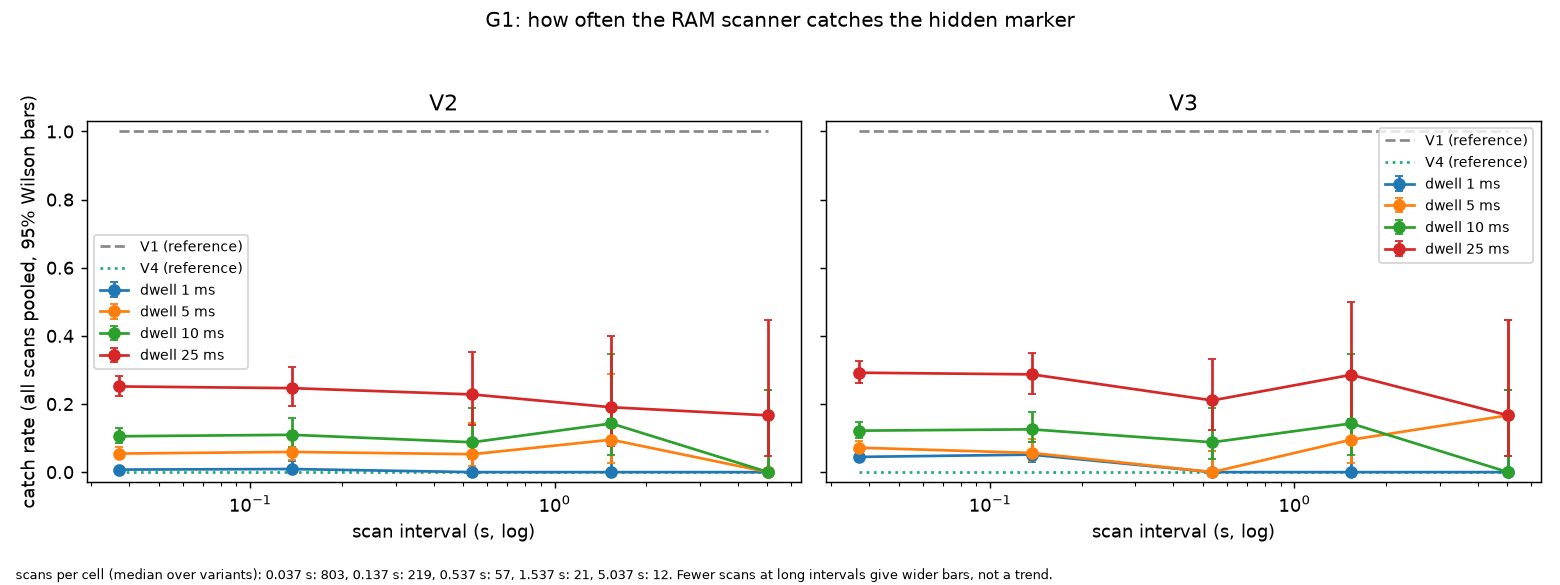
\includegraphics[width=\columnwidth]{G1_catch_rate.png}
\caption{G1: per-scan catch rate against scan interval, all scans of a cell
pooled, 95\% Wilson intervals.}
\label{fig:g1}
\end{figure}
Fig.~\ref{fig:g1}: the scanner catches V1 on every scan and V4 on none, at every
interval. For V2 the per-scan catch rate is the fraction of time a page is
exposed: 0.007, 0.055, 0.105 and 0.252 at dwell times of 1, 5, 10 and 25~ms
against 0.01, 0.05, 0.10 and 0.25 expected (about 805 pooled scans each, at the
0.037~s interval). V3 stays exposed a few milliseconds longer than its dwell: at
1~ms it is caught on 0.045 of scans (95\% interval 0.032--0.062). The rate does
not depend on the scan interval; a longer interval only delays the first catch,
and the wide bars at long intervals reflect 12 to 21 scans per cell, not a
trend. Each interval is 37~ms past a multiple of 100~ms; multiples of 50~ms
phase-lock to the payload's cycle (\#63).

\begin{figure}[t]
\centering
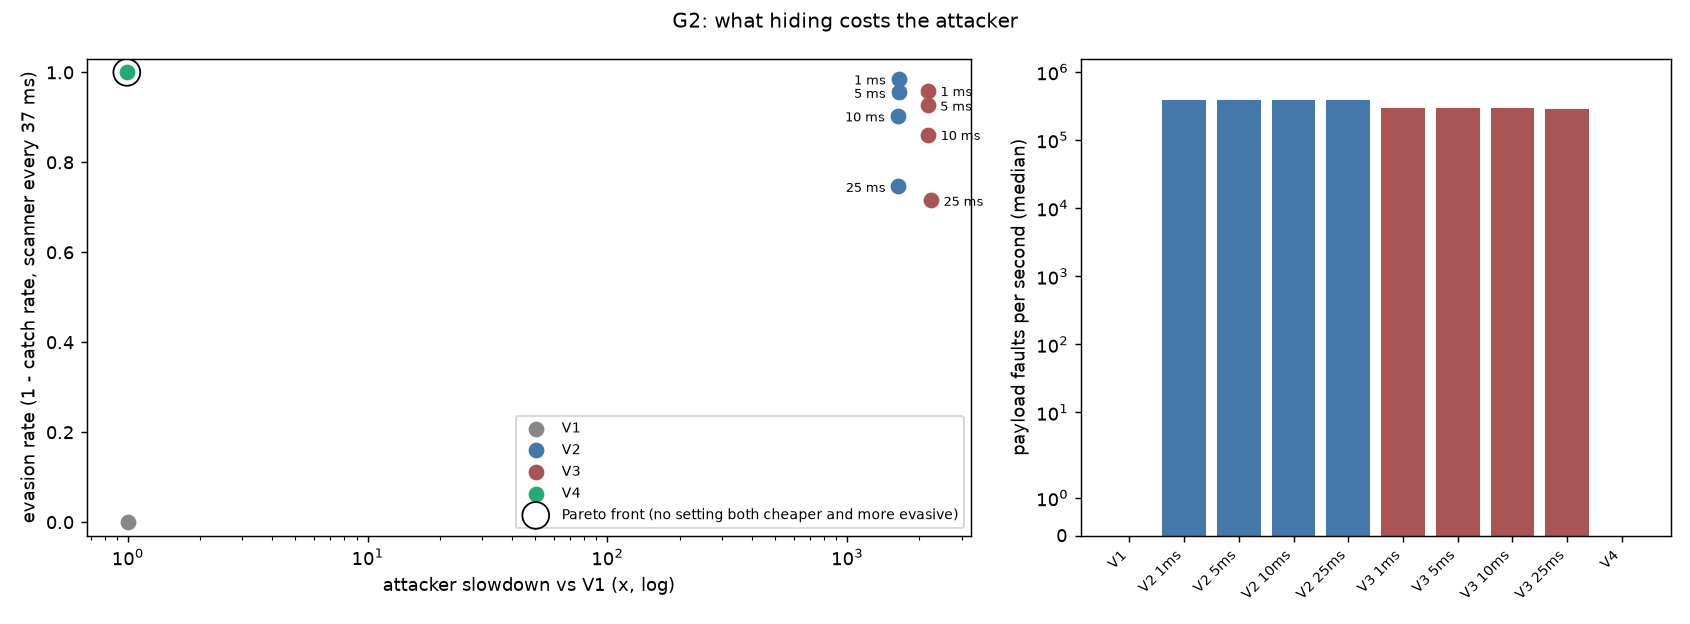
\includegraphics[width=\columnwidth]{G2_pareto.png}
\caption{G2: the attacker's slowdown against the share of scans it evades
(left), and the page faults it pays (right).}
\label{fig:g2}
\end{figure}
Fig.~\ref{fig:g2}: hiding is expensive. In a tight loop every access faults, so
V2 runs about 1,600$\times$ slower than V1 (386K faults/s) and V3 about
2,200$\times$ slower (291K faults/s), to evade 72--99\% of scans every 37~ms.
V4 evades every scan at no cost (0.99$\times$). That is the boundary of the
whole study: V1--V3 are caught only during exposure, so scheduling decides
whether they are caught; V4 defeats the scanner regardless of scheduling, and
only a syscall-level view can see it (Section~\ref{sec:det}).

\subsection{Detection-based scheduling loses to mimicry (G4)}
\begin{figure*}[t]
\centering
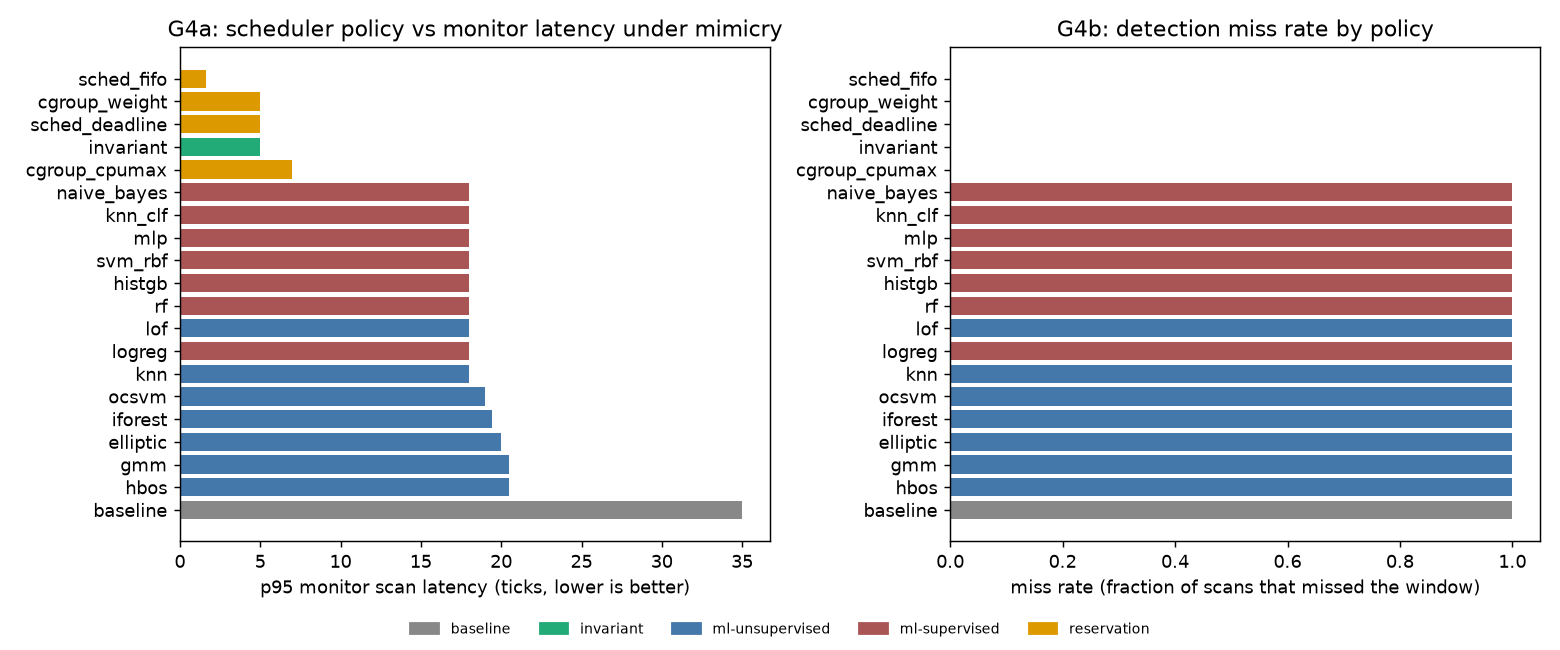
\includegraphics[width=0.66\textwidth]{G4_policy_comparison.png}
\caption{G4: monitor p95 scan latency (left) and miss rate (right) for every
policy under the coupled mimicry attack.}
\label{fig:g4}
\end{figure*}
Against the naive hog the detectors work: every ML policy ranks it perfectly
(ROC-AUC 1.00) and demotes it on at least 99\% of windows, so the monitor misses
no scan. Against the mimic, Fig.~\ref{fig:g4} shows every ML policy at a miss
rate of 1.0, the same as stock EEVDF: no scan finishes within the window (median
and interquartile range over 20 runs; single runs of three detectors dip to
0.78--0.98 when a false positive happens to demote the mimic). The
ROC-AUC explains why. The mimic sits at the center of the benign population,
while each real app is offset from it by its own jitter, so detectors that score
distance or density find the mimic \emph{more} normal than the apps it
imitates: the seven unsupervised detectors score it at 0.18--0.34 against
benign apps, and gradient boosting and the RBF-SVM at 0.28 and 0.29. Random
forest and $k$-NN vote ``normal'' for mimic and apps alike (0.50).
Logistic regression, MLP and naive Bayes rank it slightly above chance
(0.55--0.61) but far from any decision threshold: no supervised policy demoted
it on any tick of any run (0\% demotion). So 11 of the 14 score it at or below
chance, and the family median is 0.285.

\subsection{Every reservation holds; the cost frontier (G3)}
\begin{table}[t]
\caption{Reservations under the coupled attack (simulation, 20-run medians;
naive and mimicry runs are identical)}
\label{tab:frontier}
\centering
\begin{tabular}{@{}lrrrr@{}}
\toprule
Policy & p95 & Miss & Monitor & Benign \\
\midrule
\texttt{sched\_fifo} & 1.6 & 0 & 95\% & 0.6\% \\
\texttt{cpu.weight}, \texttt{deadline}, invariant & 5 & 0 & 20\% & 9.4\% \\
\texttt{cpu.max} (20\% cap) & 7 & 0 & 16\% & 64\% \\
EEVDF (reference) & 35 & 1.0 & 2.9\% & 11.4\% \\
\bottomrule
\end{tabular}
\end{table}
Every reservation keeps the miss rate at zero, under the naive hog and the mimic
alike, because none of them judges any process. Table~\ref{tab:frontier} shows
what each costs. A 25:100 \texttt{cpu.weight} split and a 0.2
\texttt{SCHED\_DEADLINE} budget give exactly the invariant's allocation in every
condition and attacker mode (bit-identical, and asserted by the test suite): the
invariant is one standard reservation, not a new mechanism. These three protect
only the monitor; the hog still takes about 71\% of the CPU.
\texttt{SCHED\_FIFO} gives the lowest latency and nearly starves the system
(0.6\% left to the benign apps). \texttt{cpu.max} is the only one that also
contains the hog (64\% left to the benign apps), but it depends on the cap: at
40\% per process the monitor misses 32\% of scans, and at 50\% all of them.

\begin{figure*}[t]
\centering
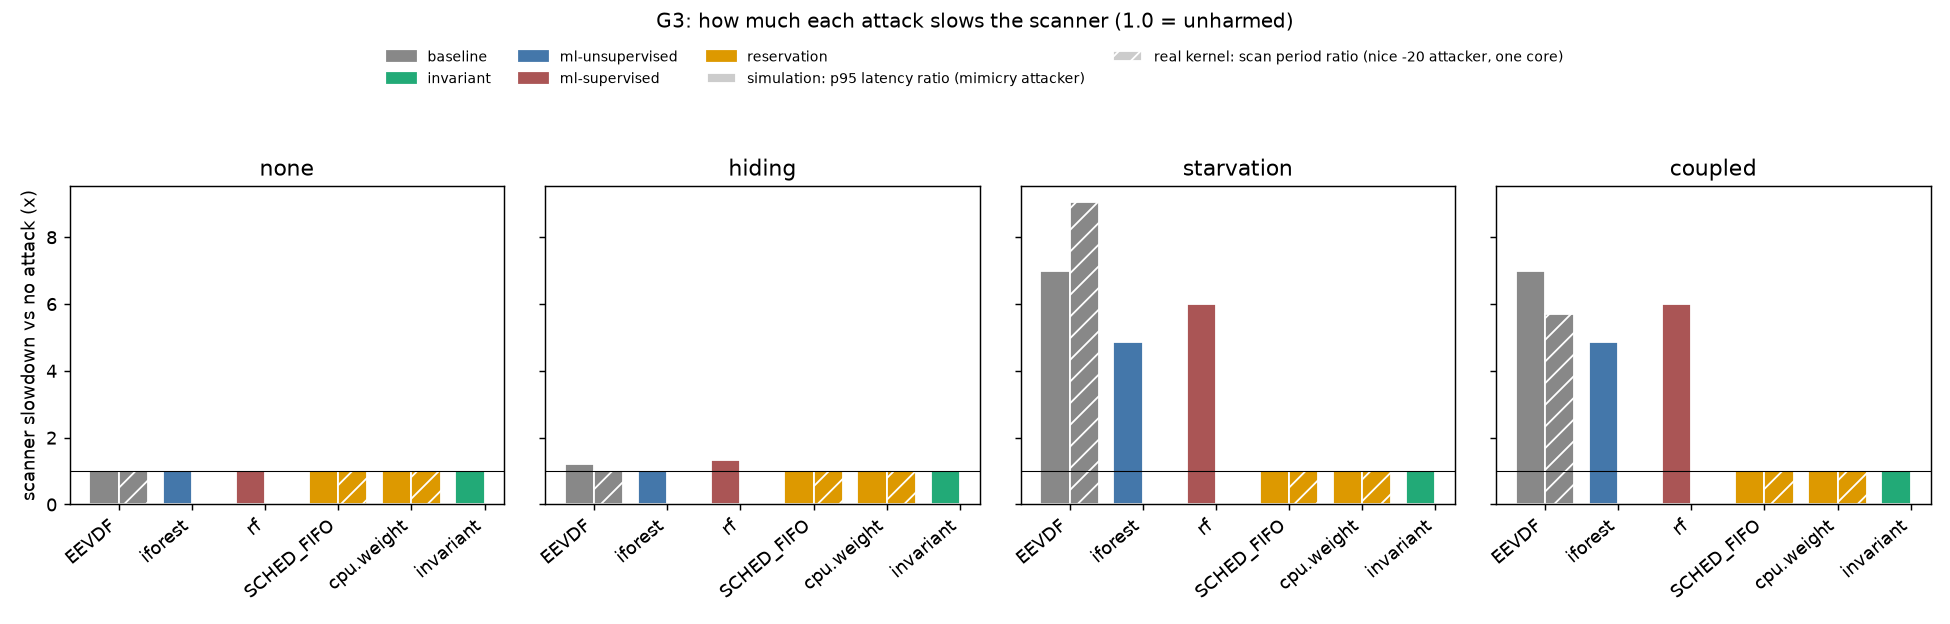
\includegraphics[width=0.94\textwidth]{G3_attack_conditions.png}
\caption{G3: scanner slowdown against no attack, per attack condition. Solid:
simulation (p95 latency ratio, mimicry attacker). Hatched: real kernel (scan
period ratio, nice $-20$ attacker on one core).}
\label{fig:g3}
\end{figure*}
Fig.~\ref{fig:g3} separates the two halves of the attack. Hiding alone barely
slows the scanner, and every reservation but \texttt{cpu.max} (up to
1.4$\times$, no miss) stays at 1.0$\times$ throughout. In the simulation, starvation and the coupled attack slow the
scanner 7.0$\times$ under EEVDF, and the ML policies do little better under
mimicry (4.9$\times$ for Isolation Forest, 6.0$\times$ for random forest).

\subsection{The reservation half on a real kernel (G3, hatched)}
On the bare-metal kernel, the scanner runs 26.75--26.95 scans/s in every
reservation cell and with no attack. Under stock EEVDF the nice~$-20$ hogs cut it
to 2.95~scans/s under starvation and 4.7 under the coupled attack (medians):
9.1$\times$ and 5.7$\times$ slower, losing 89\% and 82\% of scans. Hiding alone
costs no scans, and scan time itself never grows (p95 at most 0.42~ms): the
starvation is the scanner waiting for its turn. With \texttt{cpu.weight} or
\texttt{SCHED\_FIFO}, every condition stays at the no-attack rate. Under the
coupled attack the starved EEVDF scanner catches V2 in 15 scans (median) against
52--53 with a reservation. A control reported in the detection runs, with the
attacker at nice~0, shows no starvation, so the attack needs the claimed
priority.

\begin{table}[t]
\caption{sched\_ext: a per-PID weight in a patched \texttt{scx\_qmap} sets CPU
share (two workers on one CPU; VM)}
\label{tab:scx}
\centering
\begin{tabular}{@{}lrrr@{}}
\toprule
Phase & Attacker weight & Victim CPU & Model \\
\midrule
Equal & 100 & 49.9\% & 50.0\% \\
Attack & 2000 & 4.1\% & 4.8\% \\
Penalty & 10 & 87.6\% & 90.9\% \\
\bottomrule
\end{tabular}
\end{table}
Table~\ref{tab:scx}: a \texttt{sched\_ext} scheduler enforces per-PID weights on
a real kernel within 1--3 points of the simulation's proportional-share model,
so the weight mechanism the simulation assumes, and through which a reservation
for the scanner could be built, holds in practice.

\subsection{Detection with Tracee (G5)}\label{sec:det}
\begin{figure}[t]
\centering
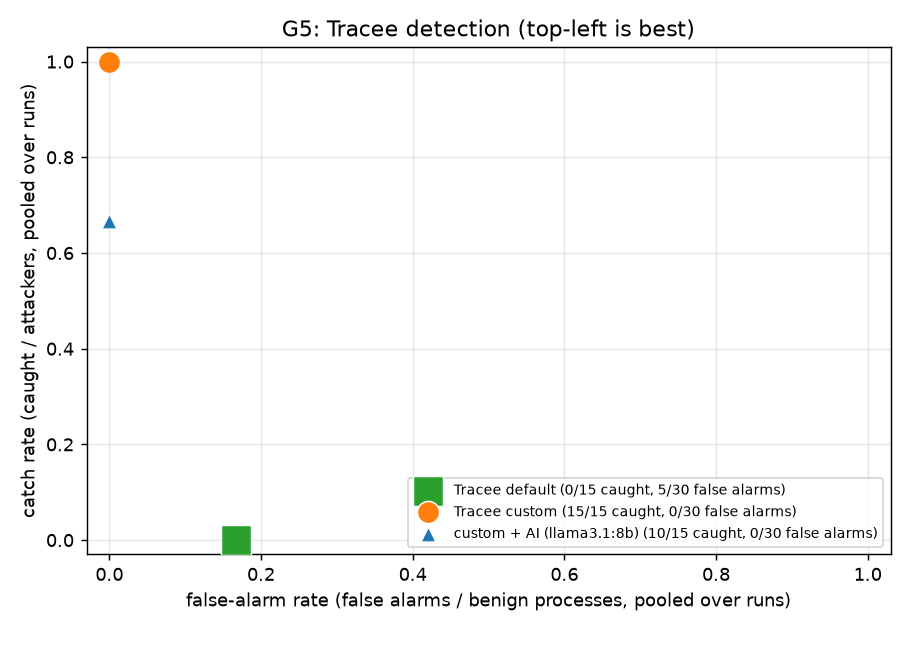
\includegraphics[width=0.85\columnwidth]{G5_detection.png}
\caption{G5: catch rate against false-alarm rate per detector, pooled over five
capture batches (15 hiding processes, 30 benign).}
\label{fig:g5}
\end{figure}
Fig.~\ref{fig:g5}: Tracee's default signatures catch none of the 15 hiding
processes and false-alarm on 5 of 30 benign ones (the JIT stand-in, every
batch). The custom rule catches all 15 with no false alarms, V4 included, which
the RAM scanner can never see: the \texttt{memfd\_secret} call itself gives it
away. Raw \texttt{PROT\_NONE} flips would not have worked: the detection runs
report Node.js making 158 and the JVM 1,413 of them without relocking any region,
while V2 made 200 round trips. AI triage of the same features catches 10 of 15, missing
one hiding process in every batch, with no false alarms. A fresh capture with
the committed script reproduces every count, batch by batch.

\subsection{What each defense costs (G6)}
\begin{figure*}[t]
\centering
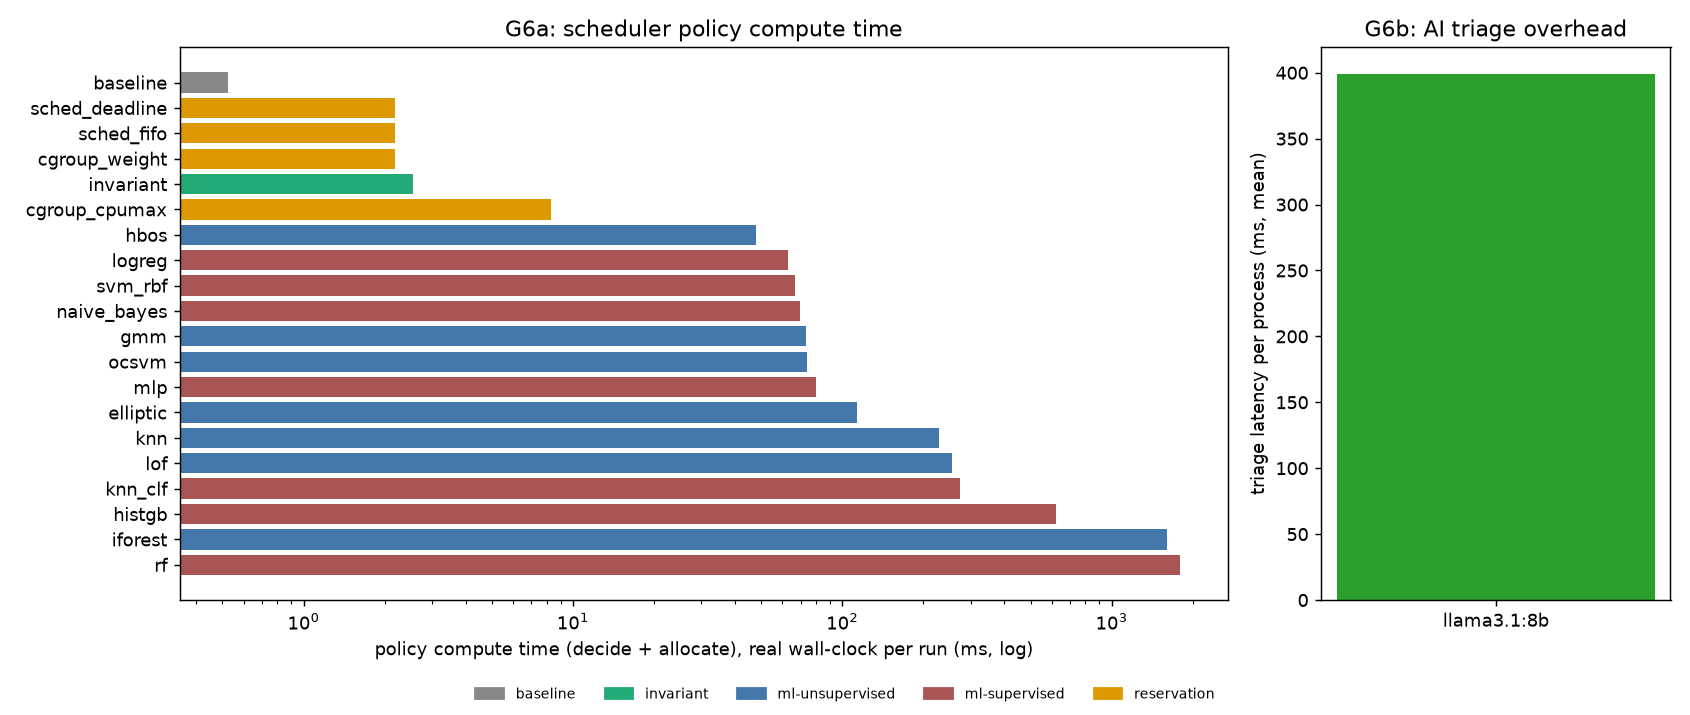
\includegraphics[width=0.66\textwidth]{G6_overhead.png}
\caption{G6: (a) single-core policy compute time per 600-tick run, deciding plus
allocating, log scale; (b) LLM triage time per process.}
\label{fig:g6}
\end{figure*}
Fig.~\ref{fig:g6}a: the reservations spend 2.2--8.3~ms of policy time per run,
the ML policies 48--1,800~ms, so a reservation is 5.8$\times$ to 826$\times$
cheaper (20-run medians). These are measured, not assumed: an earlier version timed only the
decision step, which showed the reservations at about zero by construction;
timing the allocation step too fixed that. Fig.~\ref{fig:g6}b: LLM triage adds
about 400~ms per process (317--494~ms across batches), off the scheduling path.

\section{Discussion}

\subsection{Why detection loses and reservation does not}
The mimic sits at the center of benign behavior, the least anomalous place a
process can be, so the better a detector models ``normal'', the more confidently
it waves the mimic through; training on mimics would only restart the arms race.
A reservation never asks the question: it needs to know only which process is
the monitor, which the defender controls.

\subsection{What the evidence does and does not show}
\begin{itemize}
\item The simulation is the core evidence, and its overheads are single-core
Python time, which overstates a kernel reservation's real cost (about zero per
decision).
\item The mimicry attacker exists only in the simulation, and no ML scheduler
ran on hardware. The real-kernel runs validate the reservation half: the
scanner keeps its CPU under a reservation against a high-priority hog. They do
not show detection failing against mimicry on hardware.
\item The \texttt{sched\_ext} run validates enforcement, not detection: the
penalty was applied by hand, in a VM.
\item 14 of the 15 ML policies are evaluated; the autoencoder needs the
optional PyTorch.
\item The EEVDF slowdown on hardware moved between two runs (an earlier run kept
6.0--6.2~scans/s under starvation) after the scanner and harness changed; the
cause is not established. Starved EEVDF scans also catch V2 more often (0.18 per
scan against 0.10), unexplained, so our catch loss may be a lower bound; V3's
extra exposure is unexplained too.
\item G5 is small (15 hiding and 30 benign processes, one machine, five
batches), and a hider that relocks a different address range than it unlocked
would evade the relock rule.
\item A couple of supporting observations, the nice-0 control and the Node.js
and JVM flip counts, rest on captures that were logged but not committed; every
figure and table rests on committed data.
\end{itemize}

\subsection{Corrections we made along the way}
Three claims changed under our own checks: the invariant as a unique protector
became ``every reservation protects the scanner, and the invariant is one of
them'' (\#28/\#29); the reservations' ``zero'' overhead became a measured
2--8~ms (\#55); and the first G1 sweep's phase-locked intervals were replaced
(\#63). Each correction made the result smaller and more defensible.

\section{Conclusion and Future Work}
Against an attacker that disguises its timing, scheduling that detects the
attacker fails: all 14 ML policies we evaluated miss 100\% of the scanner's
windows (median of 20 runs), because the disguised hog looks at least as benign
as the apps it imitates. A
CPU reservation that classifies no one keeps the scanner on time, and the
standard Linux primitives \texttt{cpu.weight} and \texttt{SCHED\_DEADLINE} do
it exactly as well as our invariant; on a real kernel, reservations hold the
scanner at its no-attack rate where stock EEVDF loses most of its scans. The
lesson is to sidestep the detection arms race rather than try to win it. Future
work: run a mimicry attacker against an ML \texttt{sched\_ext} policy on bare
metal, measure a \texttt{sched\_ext} reservation for the scanner alongside
\texttt{cpu.weight}, and widen the detection study to more workloads and
machines.

\begin{thebibliography}{99}
\bibitem{eevdf} I. Stoica and H. Abdel-Wahab, ``Earliest eligible virtual
deadline first: A flexible and accurate mechanism for proportional share
resource allocation,'' Old Dominion Univ., Tech. Rep. TR-95-22, 1995.
\bibitem{lwn-eevdf} J. Corbet, ``An EEVDF CPU scheduler for Linux,''
\emph{LWN.net}, Mar. 9, 2023. [Online]. Available:
\url{https://lwn.net/Articles/925371/}
\bibitem{sched-ext} The Linux kernel documentation, ``Extensible scheduler
class (sched\_ext),'' \url{https://docs.kernel.org/scheduler/sched-ext.html}.
\bibitem{cgroupv2} The Linux kernel documentation, ``Control group v2,''
\url{https://docs.kernel.org/admin-guide/cgroup-v2.html}.
\bibitem{lelli-deadline} J. Lelli, C. Scordino, L. Abeni, and D. Faggioli,
``Deadline scheduling in the Linux kernel,'' \emph{Software: Practice and
Experience}, vol. 46, no. 6, pp. 821--839, 2016.
\bibitem{memfd-secret} ``memfd\_secret(2),'' Linux manual page.
\bibitem{userfaultfd} ``userfaultfd(2),'' Linux manual page.
\bibitem{tracee} Aqua Security, ``Tracee: Runtime security and forensics using
eBPF,'' \url{https://github.com/aquasecurity/tracee}, v0.23.2.
\bibitem{wagner-mimicry} D. Wagner and P. Soto, ``Mimicry attacks on
host-based intrusion detection systems,'' in \emph{Proc. 9th ACM Conf. Computer
and Communications Security (CCS)}, 2002, pp. 255--264.
\bibitem{biggio-wild} B. Biggio and F. Roli, ``Wild patterns: Ten years after
the rise of adversarial machine learning,'' \emph{Pattern Recognition}, vol.
84, pp. 317--331, 2018.
\bibitem{tramer-adaptive} F. Tram\`er, N. Carlini, W. Brendel, and
A. M\k{a}dry, ``On Adaptive Attacks to Adversarial Example Defenses,'' in
\emph{Advances in Neural Information Processing Systems (NeurIPS)}, 2020.
\bibitem{rajkumar-resource-kernels} R. Rajkumar, K. Juvva, A. Molano, and S.
Oikawa, ``Resource Kernels: A Resource-Centric Approach to Real-Time and
Multimedia Systems,'' in \emph{Proc. SPIE 3310, Multimedia Computing and
Networking (MMCN)}, 1998.
\bibitem{iforest} F. T. Liu, K. M. Ting, and Z.-H. Zhou, ``Isolation forest,''
in \emph{Proc. IEEE Int. Conf. Data Mining (ICDM)}, 2008, pp. 413--422.
\bibitem{sklearn} F. Pedregosa \emph{et al.}, ``Scikit-learn: Machine learning
in Python,'' \emph{J. Machine Learning Research}, vol. 12, pp. 2825--2830, 2011.
\bibitem{llama3} A. Grattafiori \emph{et al.}, ``The Llama 3 herd of models,''
arXiv:2407.21783, 2024.
\end{thebibliography}

\end{document}
